%Finally, an addition step was included to the fiber conditioning process, with the objective of improving the photon collection efficiency of the fibers. 

The tritium events only produce tens of photons in the scintillating fibers, so it is very important to detect as many photons as possible. As it is demonstrated in the light collection characterization of scintillating fibers, subsection \ref{subsec:CharacterizationFibers}, the quality of the interface between the core of uncladded fibers and the environment (tritiated water in the case of TRITIUM detector) affects conspicuously the photon collection efficiency. To improve the quality of the interface, a fiber cleaning process was implemented, aiming to remove external particles deposited on the fibers, such as dust and fat that worsen the photon collection efficiency.  Through this cleaning process, the wetting property of the fibers is improved, that is to say the capacity of its surface to attract water, as illustrated in Figure \ref{fig:WettingProperty}. This implies an increase of the contact surface between the fibers and water, which prevents air molecules from attaching to them, and produces a uniform water clad around them.

%Therefore, a mechanism, called the fiber cleaning process, was applied. As we can see in Figure \ref{fig:WettingProperty}, this cleaning process was carried out to improve the wetting properties, preventing air molecules from attaching to the fiber and achieving a uniform water clad around each fiber, avoiding variations in its refractive index which can worsen the photon collection efficiency of the fibers.

\begin{figure}[h]
\centering
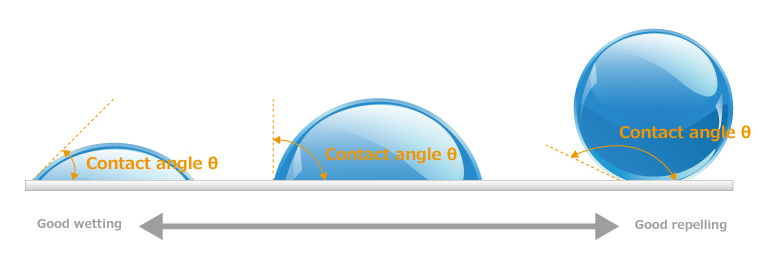
\includegraphics[scale=0.5]{4ResearchAndDevelopments/41Fibers/WettingProperty.png}
\caption{Schematic representation of the wetting properties of a flat surface (gray) in contact with a drop of liquid (blue). The wetting property is characterized by the angle formed between the surface of both objects. The smaller angle, the better wetting property of the material. \cite{WettingProperty}\label{fig:WettingProperty}}
\end{figure}

This cleaning process  was developed and carried out in the clean room of ICMOL laboratory. Three different glass beakers were used, one filled with alkaline soap, another with pure water (conductivity of the order of $10~\mu\text{S}/\cm$) and the third with isopropanol. The fibers are first rubbed with gloved hands with alcalin soap during 5 minutes, then placed in the first beaker which is placed in an ultrasonic bath at $17~\kilo\hertz$ frequency during 3 minutes. Then, the fibers are cleaned with a constant flow of water during 5 minutes and they are placed in the second beaker for ultrasonic bath during 3 minutes and then placed in the third beaker for ultrasonic bath during another 3 minutes. Finally the fibers are dried with a flow of gas $\ce{N_2}$ and kept in clean conditions until their introduction into the module vessel of TRITIUM detector.

The improvement in the light collection of the scintillation fibers after this cleaning process was measured using a bundle of twenty uncladded fibers of $15~\cm$ length that have undergone this cleaning process. This bundle of fibers was arranged in the setup described in Figure \ref{fig:BunchWith2PMTsCoincidence} and the energy spectra were measured, before and after cleaning the fibers. Similar to the polishing machine test, this measurements was done first for the background, Figure \ref{fig:ResultsOfCleaningProcessBackground}, and then using two radioactive sources; a $\ce{^{90}Sr}$ beta source, already used in the polishing machine test, and an encapsulated $\ce{^{137}Cs}$ source with gamma emisions of $661.7~\keV$ and an activity of $500~\becquerel$ activity, Figures \ref{fig:ResultsOfCleaningProcessSource}. A higher gain was used in this case to optimize the number of channels used of the MCA (the digital multichannel analizer). A shift of the spectrum to higher energies is observed in all the cases for the clean fibers, with respect to the spectra obtained before cleaning, showing an improvement in photon collection efficiency of the fibers. A similar equation to \ref{eq:RelativeImprovement} was used  quantify the improvement achieved with the cleaning process. Although no improvement in the detected events was observed for the background measurement, an improvement of about $26\%$ and $35\%$ was obtained for $\ce{^{90}Sr}$ and $\ce{^{137}Cs}$ respectively.

\begin{figure}[h]
\centering
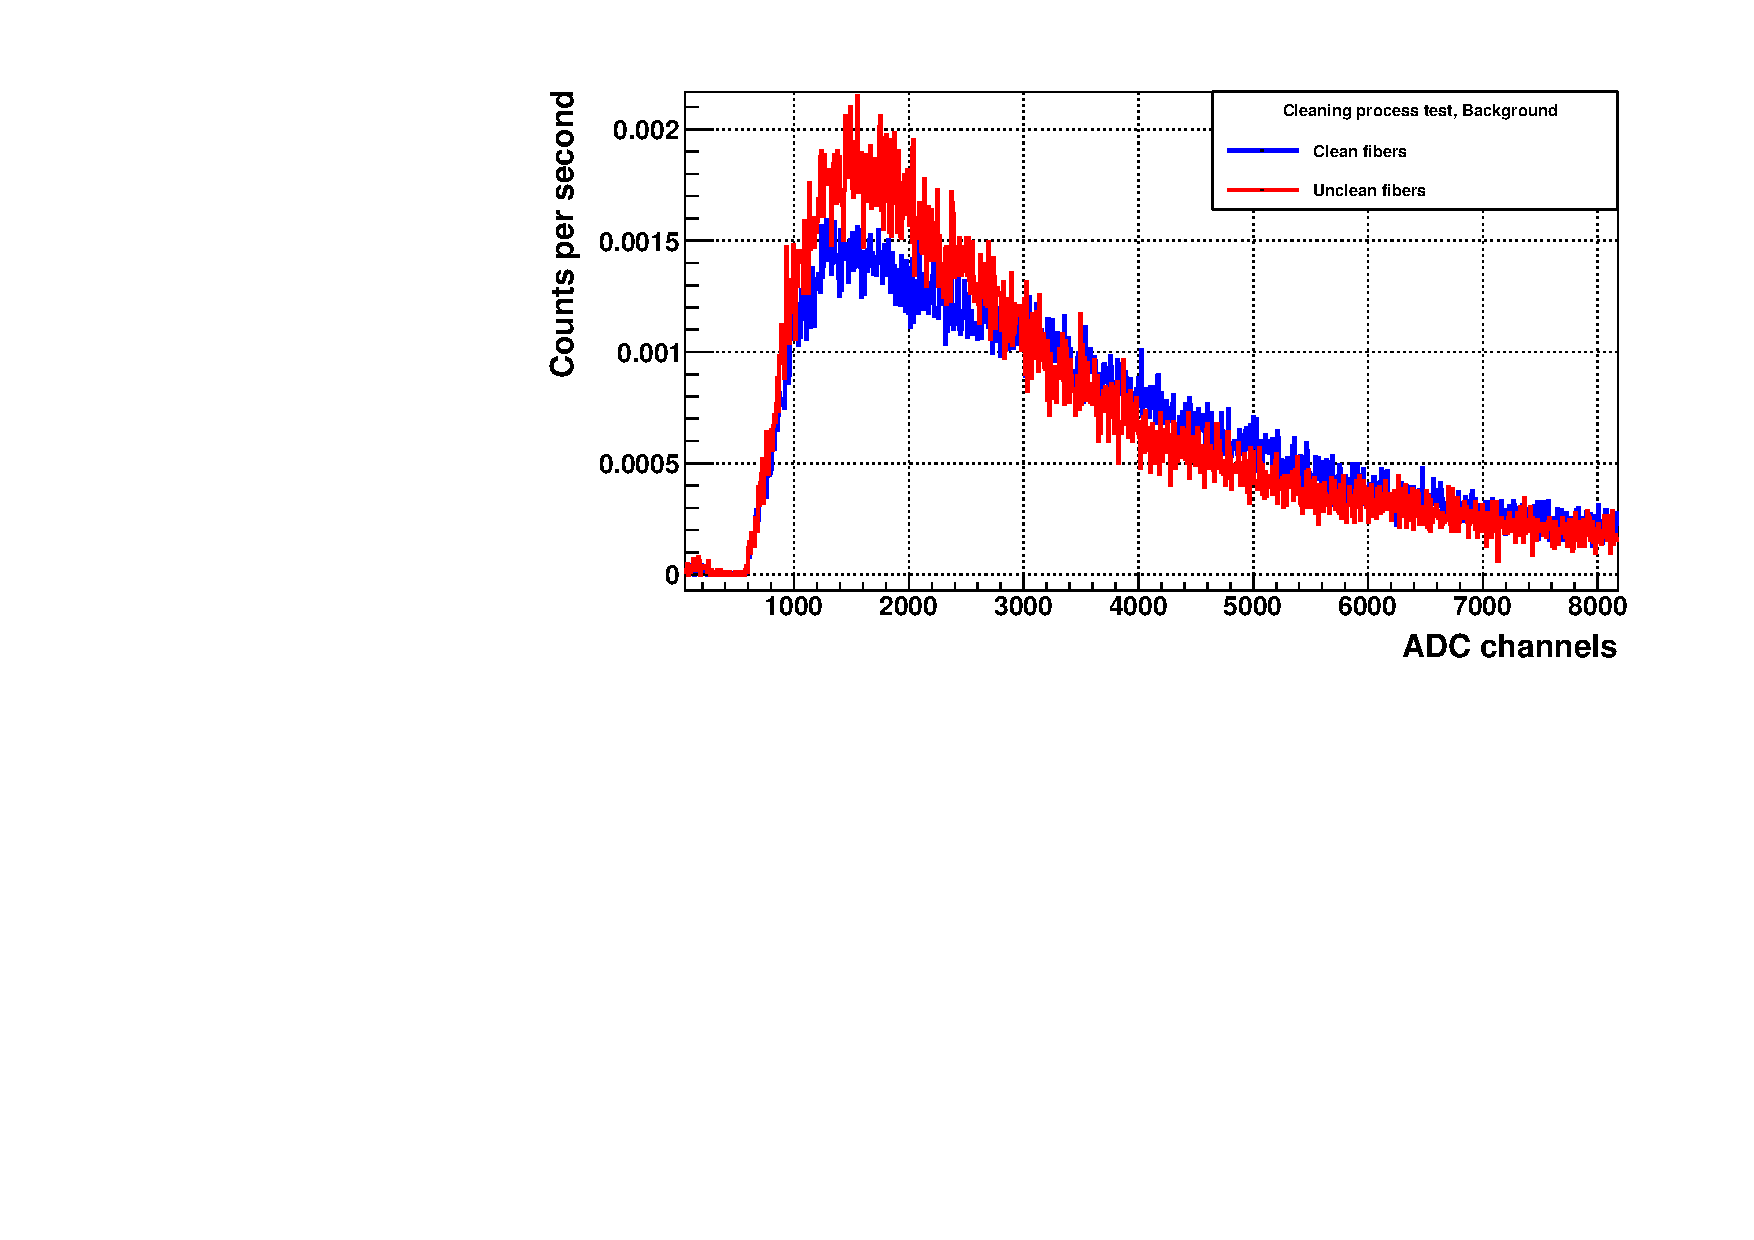
\includegraphics[scale=0.6]{4ResearchAndDevelopments/41Fibers/Background_CleaningProcess.pdf}
\caption{Energy spectra of the background before and after the cleaning process.\label{fig:ResultsOfCleaningProcessBackground}}
\end{figure}

\begin{figure}
\centering
    \begin{subfigure}[b]{1\textwidth}
    \centering
    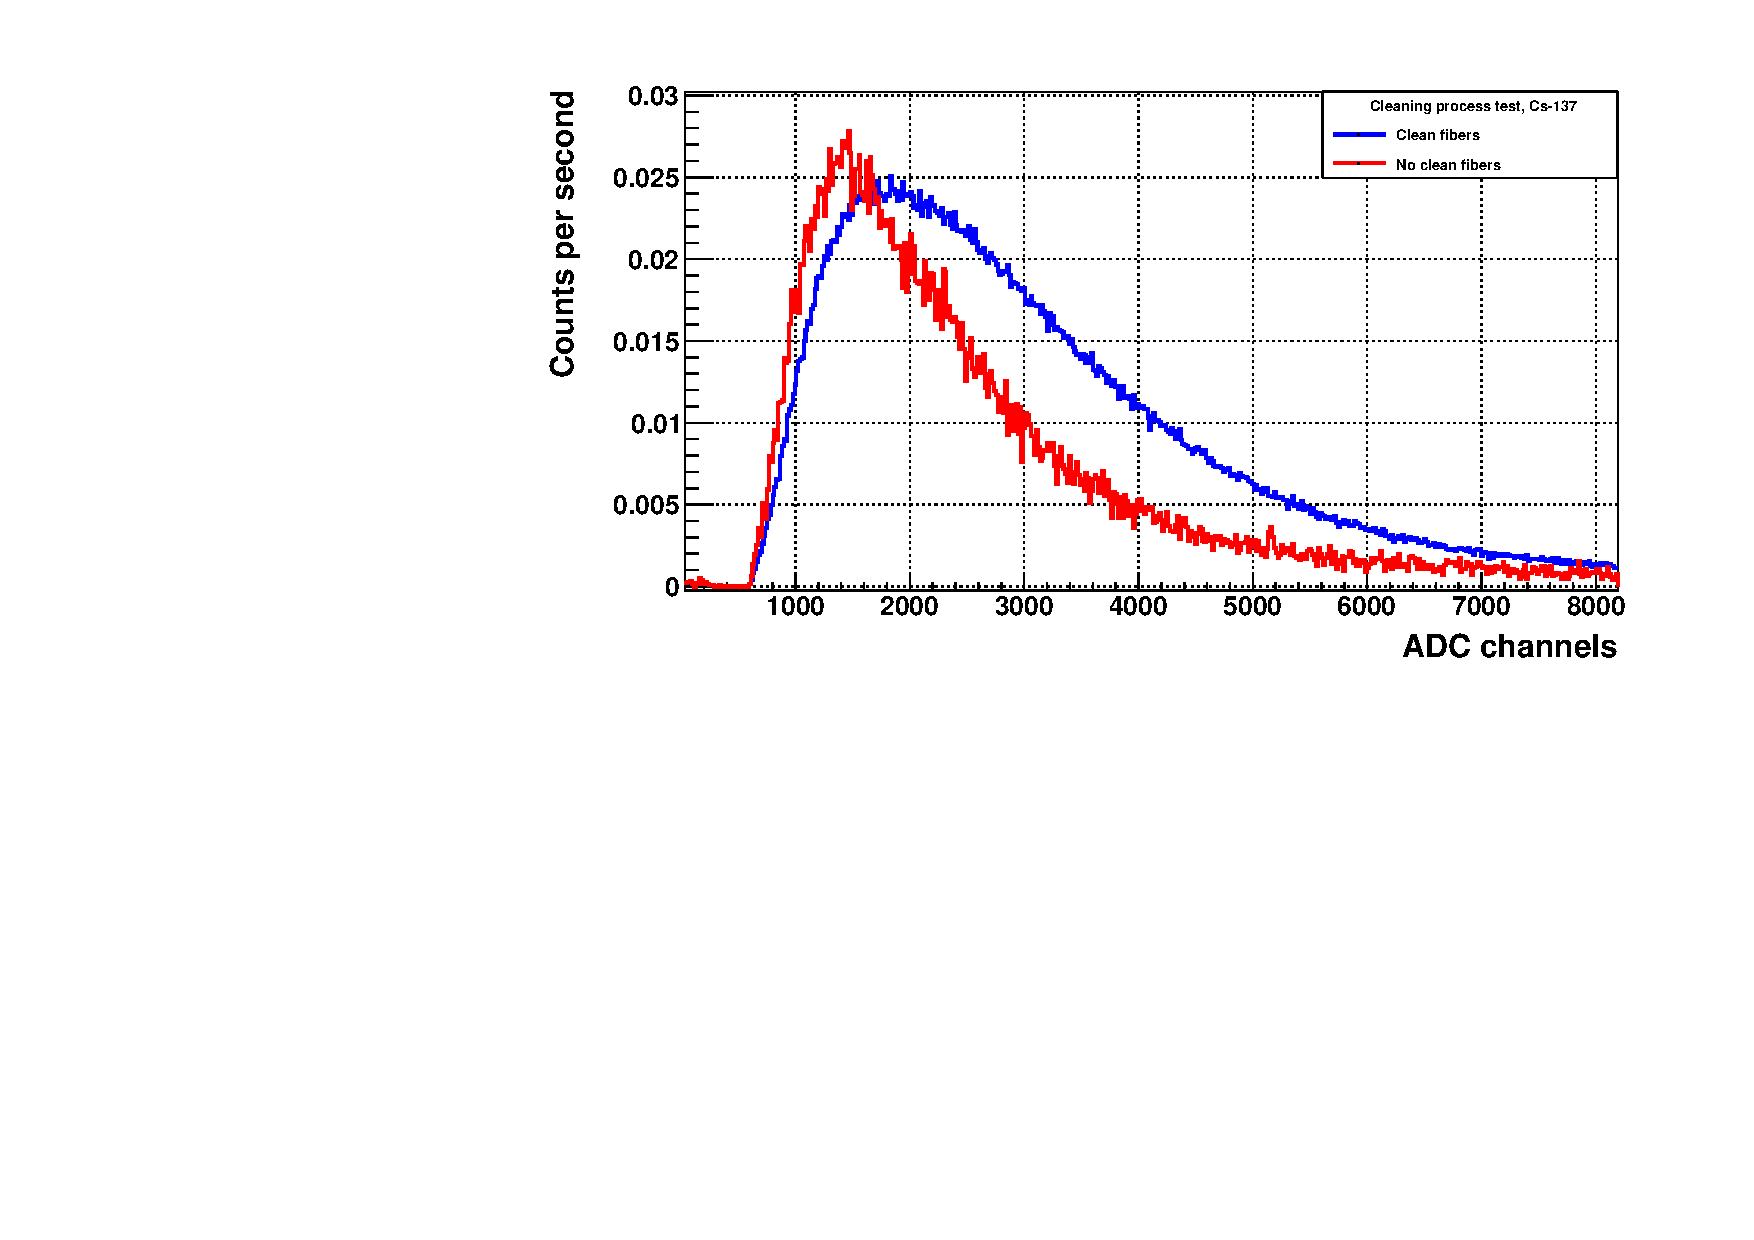
\includegraphics[width=\textwidth]{4ResearchAndDevelopments/41Fibers/Cs-137_CleaningProcess.pdf}  
    \caption{\label{subfig:EnergySpectrumCo60CleaningTest}}
    \end{subfigure}
    \hfill
    \begin{subfigure}[b]{1\textwidth}
    \centering
    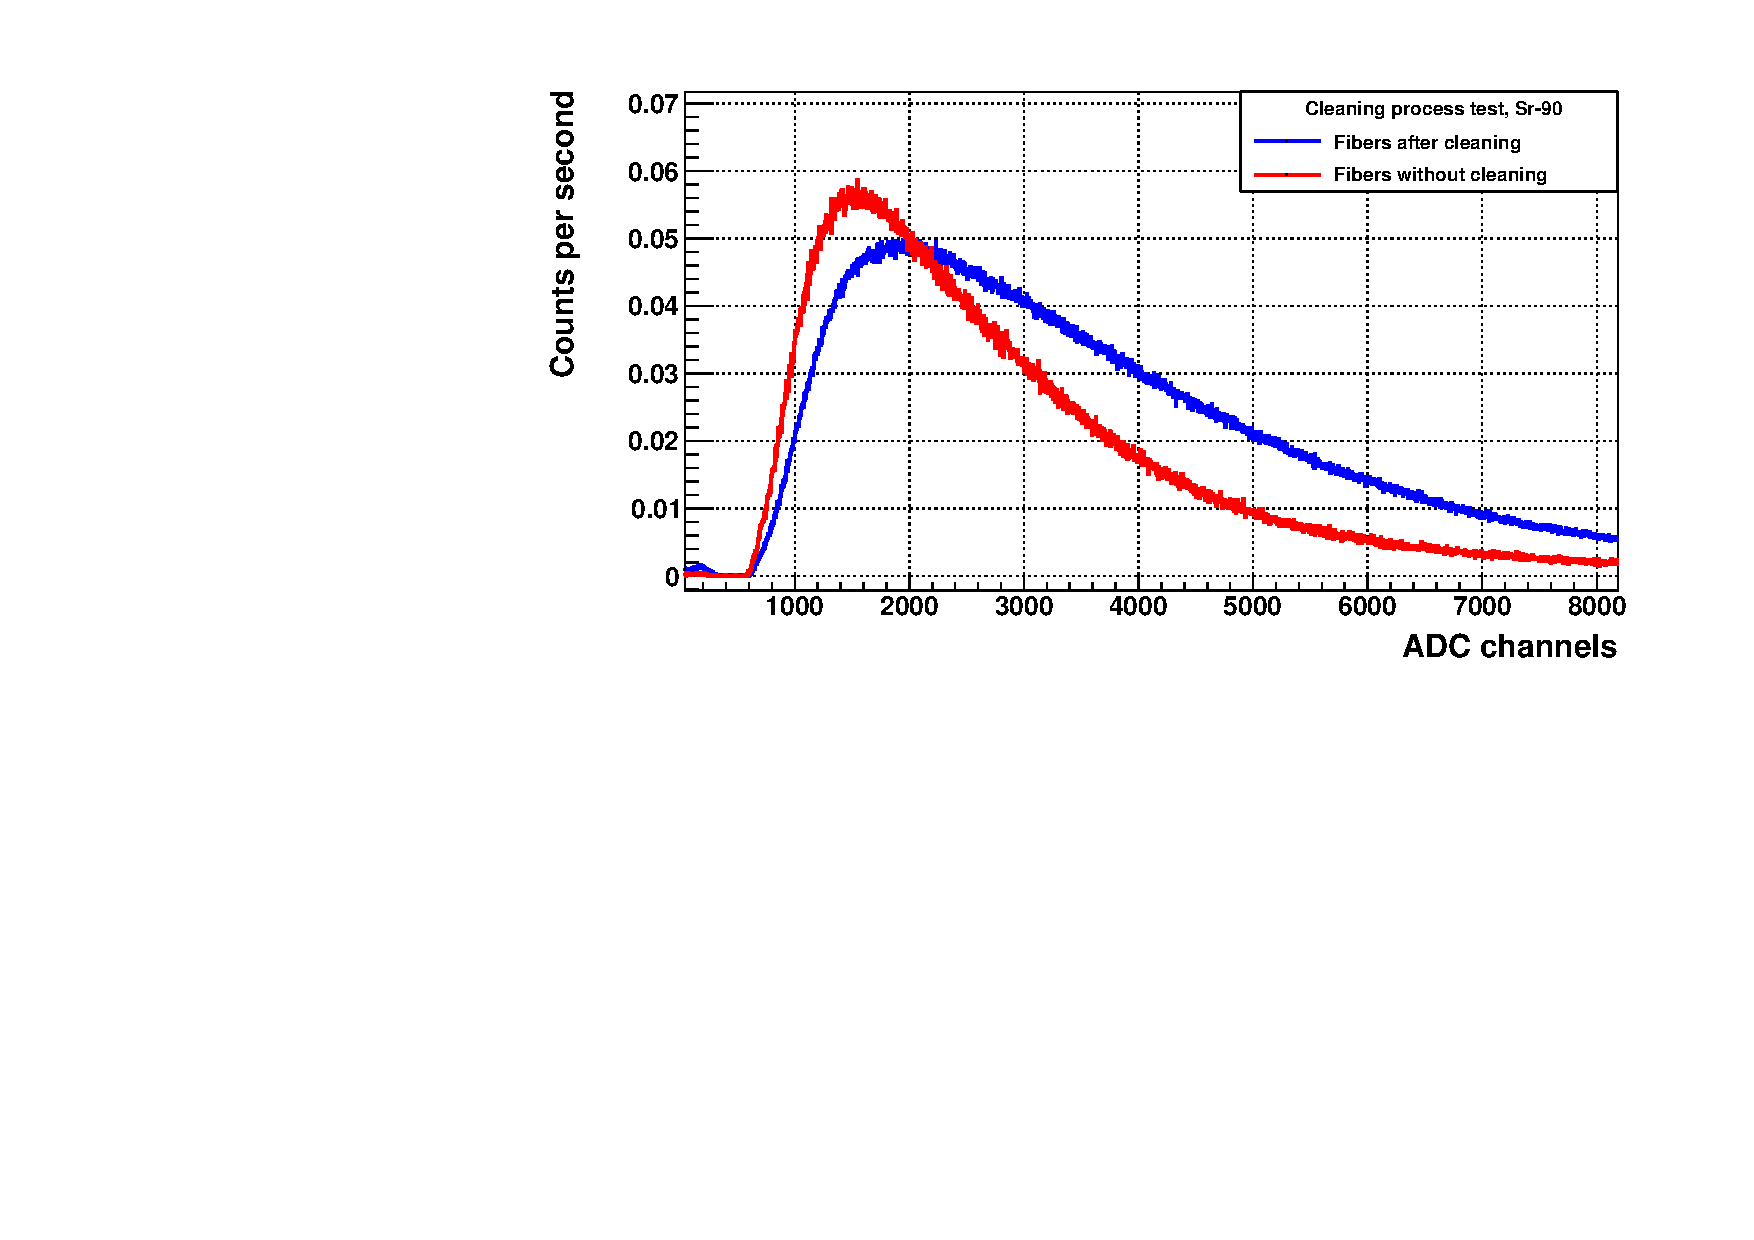
\includegraphics[width=\textwidth]{4ResearchAndDevelopments/41Fibers/Sr-90_CleaningProcess.pdf}  
    \caption{\label{subfig:EnergySpectrumSr90CleaningTest}}
    \end{subfigure}
 \caption{Energy spectra obtained before and after the cleaning process using a radioactive source of a) $\ce{^{137}Cs}$ and b) $\ce{^{90}Sr}$.}
 \label{fig:ResultsOfCleaningProcessSource}
\end{figure}


%$(27.73 \pm 1.6)\%$ for the gamma source and $(20.72 \pm 0.9)\%$ for the beta source so, the improvement of the photon collection efficiency of the fibers was verified using the cleaning process carried out in the clean room of ICMOL laboratories. Nevertheless, it should be taken into accout that this test was carried out in air. It could be interesting to repeat it in water to obtain more realistic conclusions since the fibers of the TRITIUM detector will be immersed in water.